\chapter{Introduction}
\section{Motivation}
\vspace{-0.1cm}
Thanks to recent advancements in Artificial Intelligence (AI), we are now able to leverage Machine Learning and Deep Learning technologies in both academic and commercial applications. Although, relying just on correlations between the different features, can possibly lead to wrong conclusions since correlation does not necessarily imply causation.

Three of the main limitations of nowadays Machine Learning and Deep Learning models are: 
\vspace{-0.2cm}
\begin{itemize}
    \item \textbf{Robustness}: trained models might not be able to generalise to new data and therefore would not be able to provide robust and reliable performances in the real world.
    \item \textbf{Explainability}: complex Deep Learning models can be difficult to analyse in order to clearly demonstrate their decision making process. 
    \item \textbf{Data Dependency}: deep learning models efficiency is highly dependent on the amount and quality of data available. 
\end{itemize}
\vspace{-0.2cm}
Developing models able to identify cause-effect relationships between different variables, might ultimately offer a solution to solve these problems. This idea, has also been supported by researchers such as Judea Pearl and Jonas Peters, which advocated how having models able to reason in uncertainties could not be enough to enable researchers to create machines able to truly express intelligent behaviour \cite{art_perl}.

\section{Going Beyond Correlation}
\label{simp_ref}
Paradoxes are a classes of phenomena which arise when, although starting from premises known as true, we derive some sort of logically unreasonable result. One of the most common form of paradox in Data Science is \textbf{Simpson's Paradox}.

As an example, let us consider a thought experiment. We carried out a research study in order to find out if doing daily physical exercises can help or not reduce Cholesterol levels (in mg/dL) and we are now starting to examine the obtained results. First, we divide our population sample into two main categories based on the individuals age (under/over 60 years old) and then we plot their cholesterol levels against the number of hours the subjects exercised per day. By examining the results in the first two plots of Figure \ref{s1}, we can then infer that exercising for more hours a day can then lead to an overall reduction in our cholesterol levels. This hypothesis can then also be reinforced by examining the overall trend of the best fit line inferred through Linear Regression and the quite strong negative Person Correlation scored in both cases. At this point, comforted by our derived results, we can then try to repeat this same analysis taking into consideration this time the whole population sample (rightmost plot in Figure \ref{s1}). In this case, we are faced with a completely contradictory scenario and a positive correlation implying that more exercise can lead to increased cholesterol levels.

\begin{figure}[ht!]%
    \centering
    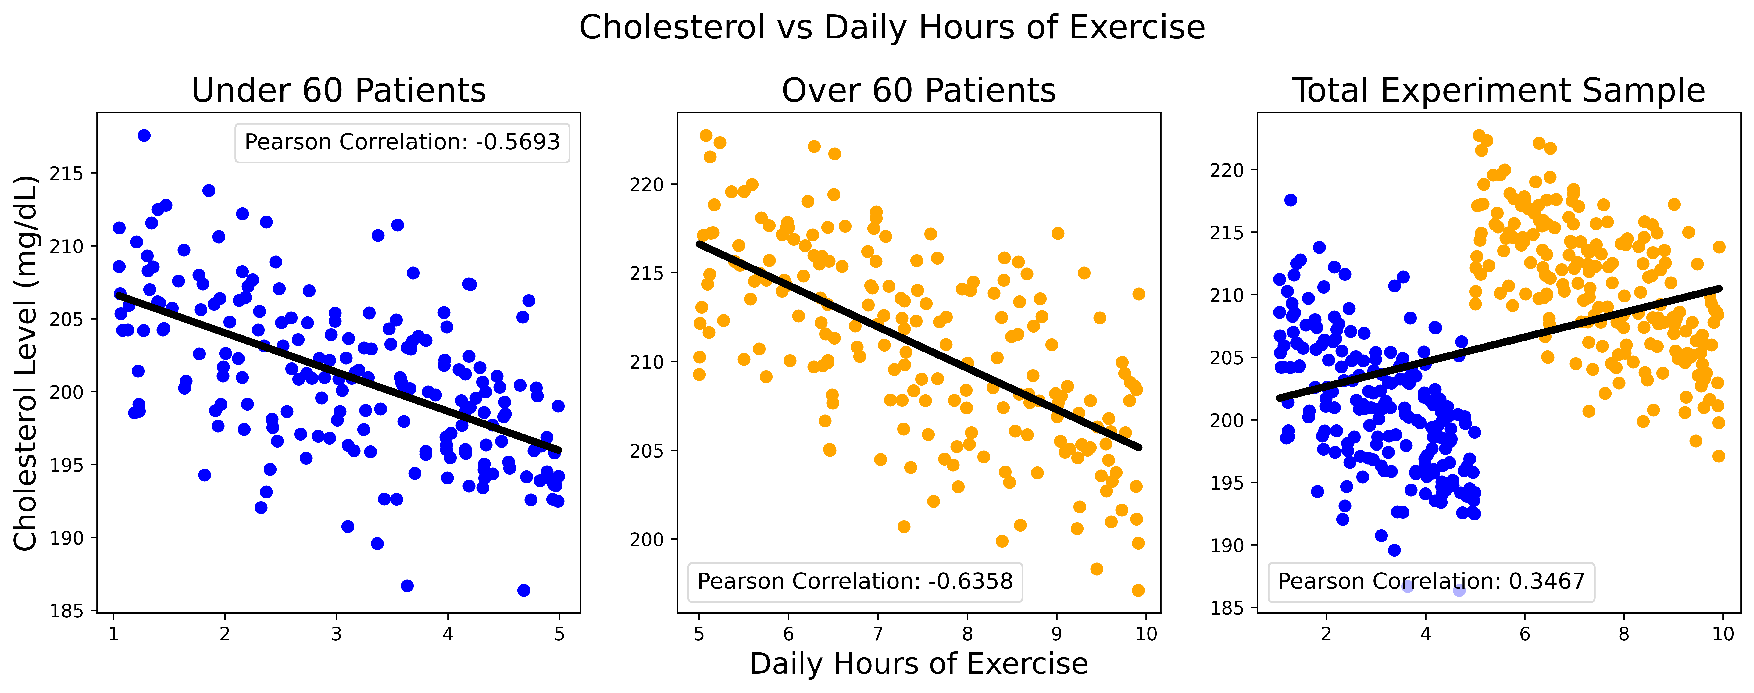
\includegraphics[width=1\linewidth]{latex/images/simpson1.pdf}
    % 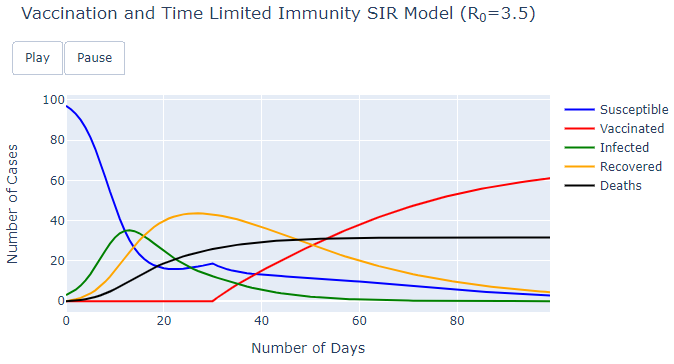
\includegraphics[width=13cm]{latex/images/vacc.PNG}%
    \vspace{-0.5cm}
    \caption{Cholesterol vs Daily Hours of Exercise}
    \label{s1}
\end{figure}
\vspace{-0.7cm}

This type of scenario is commonly known as Simpson's Paradox and takes place everytime we have some form of correlation which points in a direction when considered in a sub-group and points instead in the opposite direction if considered as part of the whole group. In order to unveil the reasons behind this type of mechanism, we need to try to go beyond the provided data and think about how our data was generated in the first place to \textbf{cause} this outcome (e.g. What unknown missing variable might be preventing us to see the full picture?).

In this simple scenario, our missing component could be any potentially influential variable such as: individual's comorbidities, diet and age. We decide then to take a closer look on how cholesterol levels vary with greater age (Figure \ref{s2}). Repeating the same analysis done in Figure \ref{s1}, we can then clearly see how cholesterol levels are strongly positively correlated to individual's age.

\begin{figure}[ht!]%
    \centering
    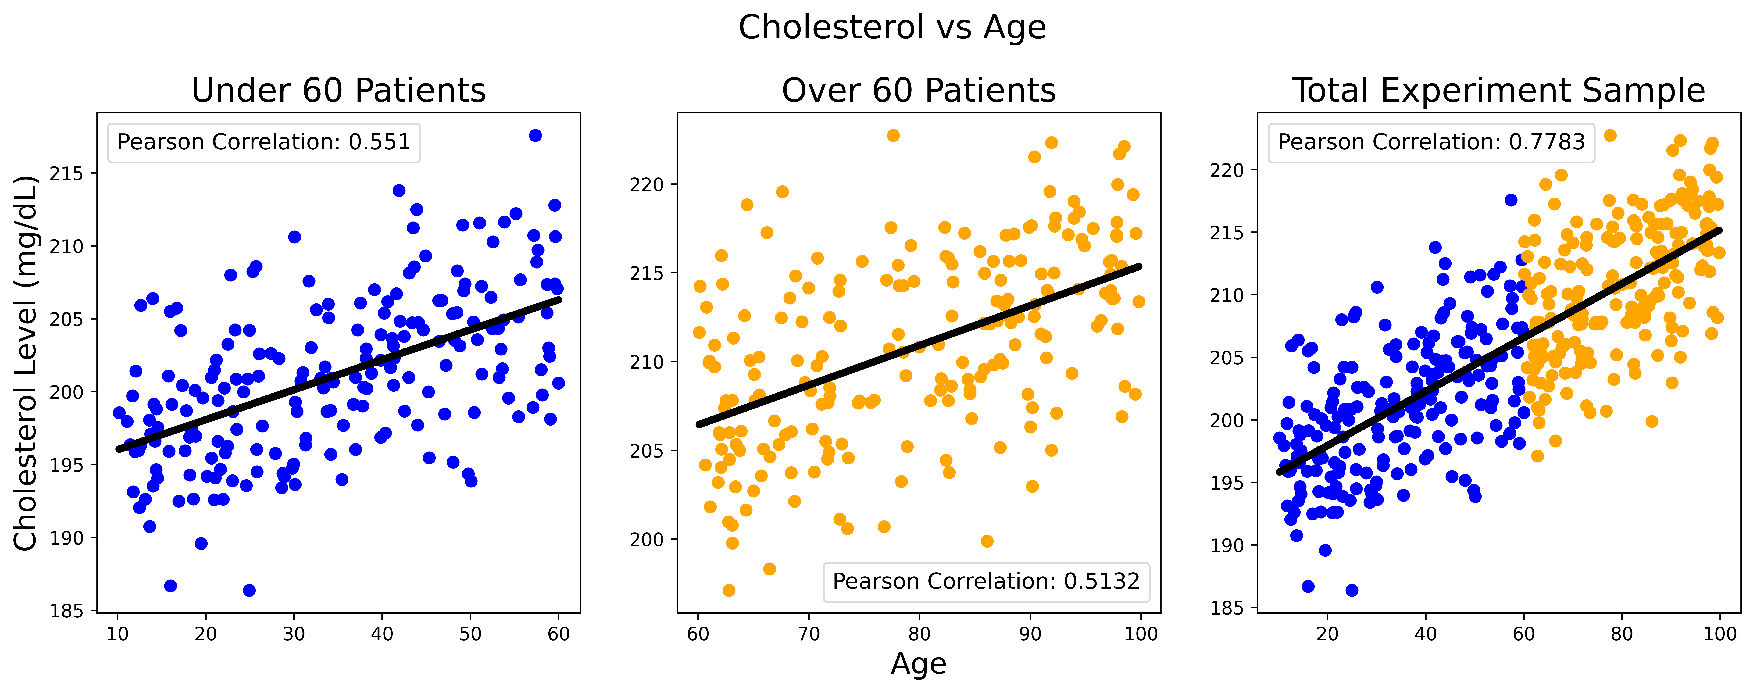
\includegraphics[width=1\linewidth]{latex/images/simpson2.pdf}
    % 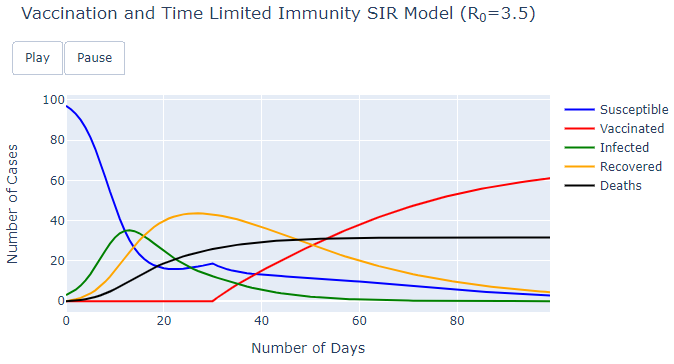
\includegraphics[width=13cm]{latex/images/vacc.PNG}%
    \vspace{-0.2cm}
    \caption{Cholesterol vs Age}
    \label{s2}
\end{figure}

From these results, we can then deduce that cholesterol levels are more likely to increase with aging and lack of exercise (there is cause effect relationship between the three variables). Therefore, in order to try to quantify the benefits of exercising in reducing cholesterol levels and overcome the Simpson Paradox, we should then make sure to run our experiment while having a fixed value for the age of the subjects (\textbf{controlling the variable}).   

During the course of the last century, the Simpson Paradox occurred in many statistical studies such as: UC Berkeley gender bias, Kidney stone treatment and Racial disparity in the death penalty \cite{simpara}. Other common examples of statistical/mathematical paradoxes are the Monty Hall Problem, the Berkson's Paradox and the Accuracy Paradox.

Additional information about technical limitations of correlation and possible alternative metrics which have been designed in order to overcome this type of problems is available in Appendix \ref{pps}.

\section{Causality vs Explainability}
One of the major trade-offs in nowadays Machine Learning is model performance against complexity. In fact, complex Deep Learning architectures are usually able to perform better in a wide variety of tasks compared to traditional linear classifiers and regression techniques. This trade-off has been analysed in-depth in the 2016 publication "Why should I trust you?" by Ribiero et. al. \cite{otto} and led a new trend in AI to focus on interpretability.

Complex and more accurate models are nowadays referred to as \textbf{Black-boxes}. These type of models working progresses are more difficult to comprehend and they are not able to estimate the importance of each feature and how they are related to each other. Some examples of Black Boxes models are neural networks and ensemble models.

On the other hand, simpler and less accurate models such as decision trees and linear regression, are instead regarded as \textbf{White-boxes} and can be much more interpretable. Two of the main measures which can be used in order to estimate the explainability of a model, are the linearity and monotonicity of a model response function \cite{nove}.

One of the key differences between Explainable AI and Causal AI, is that the former aims just to understand how a model might come to a prediction by weighting the provided features while the latter is designed undercover the process governing the system we are analysing to create insights. In this way, Causal AI can be used in order to answer common retrospective and system design type of questions, providing vital business value to organizations (e.g. EU’s General Data Protection Regulation, right to explanation clause) \cite{causalens}.

\section{Foundations of Modelling and Simulations}
Modelling and Simulations is a branch of mathematics which aim to be able to imitate real-world processes over a period of time. In this way, artificially generated historical data can be easily created and used in order to make inference in real-world applications. Simulation models are usually based on a series of simplifying assumptions (of the real-world environment) which can then be expressed in a mathematical or symbolic notation \cite{mod_1}. 

There are two main types of programmable simulation models:
\begin{itemize}
    \item \textbf{Mathematical Models}: makes use of mathematical symbols and relationships in order to summarise processes. Compartmental Models in Epidemiology are a typical example of mathematical models.
    \item \textbf{Process Models}: are based on list of steps handcrafted by the designer in order to represent an environment (e.g. Agent Based Modelling).
\end{itemize}

Modelling and Simulations, are nowadays used in many different fields such as Finance (e.g. Monte Carlo Simulations for Portfolio Optimization), Medical/Military Training, Epidemiology and Threat Modeling \cite{mod_2, mod_3}. 

Some of the main uses of simulations is to verify analytical solutions, experiment policies before creating any physical implementation and understand the connection and relative importance of the different variables composing a system (e.g. by modifying input parameters and examining the results). These properties, makes therefore the Modelling and Simulations paradigm a \textbf{white-box} approach to predict future trends.

\section{Objectives}
\vspace{-0.1cm}
As part of this research study, will be outlined the main principles of Causal Reasoning and different application approaches (e.g. Bayesian Belief Networks, Time Series Analysis) and an Epidemic Modelling case study concerning COVID-19 (Coronavirus). 

The Novel Coronavirus, is new type of RNA virus which can be able to infect humans potentially causing respiratory infections. The 2020 Novel Coronavirus outbreak started in the late 2019 in Wuhan, China and, as of July 2020, it is believed the virus is mainly able to spread by air through sneezing and coughing. 

The proposed Compartmental Models, will be based on paradigms defined in the Epidemiology literature \cite{adam_k} and the Imperial College of London COVID-19 report studies used by the UK government in order to handle the outbreak \cite{mod_4}. The Agent Based Models have instead been handcrafted in order to provide an alternative approach to traditional mathematical model implementations including different elements of stochasticity due to non-linear interactions at a population level. 

Due to the design of the proposed models, they can potentially provide greater help for decision makers (compared to traditional Machine Learning approaches), if and only if, the decision makers in question have the necessary understanding of epidemiology and its key control metrics. 

Finally, these models have been exclusively designed for educational and research purposes and are not to be applied in any other ambit (e.g. commercial, governmental).

